\documentclass[a4paper]{article}
\usepackage[english]{babel}
\usepackage[utf8]{inputenc}
\usepackage{fancyhdr}
\usepackage{hyperref}
\usepackage{amsmath,amsfonts,amssymb,amsthm}
\usepackage[a4paper, bottom=1.3in, top=1.3in, right=1in, left=1in]{geometry}
\usepackage[usenames,dvipsnames]{xcolor}
\usepackage{tikz}
\definecolor{amaranth}{rgb}{0.9, 0.17, 0.31}
\usepackage{graphicx}
\usepackage{caption}
\usepackage{subcaption}
\usepackage{layouts}


%%%%%%%%%%%%%%%%%%%%%%%%%%%%%%%%%%%%%%%%%%%
% Insert your name here
\newcommand{\fullname}{Clément Bonnet}
%%%%%%%%%%%%%%%%%%%%%%%%%%%%%%%%%%%%%%%%%%%

\newcommand{\lecture}[3]{
   \pagestyle{myheadings}
   \thispagestyle{plain}
   \newpage
   \setcounter{page}{1}
   \noindent
   \begin{center}
   \framebox{
      \vbox{\vspace{2mm}
              \hbox to .97\textwidth { {\bf MVA: Reinforcement Learning (2020/2021) \hfill Homework 1} }
       \vspace{6mm}
       \hbox to .97\textwidth { {\Large \hfill #1 \hfill } }
       \vspace{6mm}
       \hbox to .97\textwidth { {Lecturers: \it A. Lazaric, M. Pirotta  \hfill {{\footnotesize(\today)}}} }
      \vspace{2mm}}
   }
   \end{center}
   Solution by {\color{amaranth}\fullname}
   \markboth{#1}{#1}
   \vspace*{4mm}
}


\DeclareMathOperator*{\argmax}{\arg\,\max}
\DeclareMathOperator*{\argmin}{\arg\,\min}
\DeclareMathOperator*{\arginf}{\arg\,\inf}
\DeclareMathOperator{\sign}{sign}


\setlength{\parindent}{0cm}
\begin{document}
\lecture{Dynamic Programming}{1}


\pagestyle{fancy}
\fancyhf{}
\rhead{Full name: {\color{amaranth}\fullname}}
\lhead{Dynamic Programming}
\cfoot{\thepage}



\section{Question}

\subsection{}

Finding the shortest path to state 14 corresponds to a deterministic policy. The reward $r_s$ has to be negative to ensure the shortest path goal while not being too low to prevent the agent from visiting red terminal state 1. Precisely, $r_s$ must respect: $-10 < r_s < 0$.

Let us define $\boxed{r_s = -1}$. Since the transitions are deterministic, the optimal policy is indeed the shortest path to state 14. For such rewards, the value function of the optimal policy for each state is the following.

\begin{center}
\tikz{
    \draw[very thin] (0,0) rectangle (1,1) node[pos=.5] {8};
    \draw[very thin] (0,1) rectangle (1,2) node[pos=.5] {7};
    \draw[very thin] (0,2) rectangle (1,3) node[pos=.5] {6};
    \draw[very thin] (0,3) rectangle (1,4) node[pos=.5] {5};
    \draw[very thin] (1,0) rectangle (2,1) node[pos=.5] {9};
    \draw[very thin] (1,1) rectangle (2,2) node[pos=.5] {8};
    \draw[very thin] (1,2) rectangle (2,3) node[pos=.5] {7};
    \draw[fill=red, very thin] (1,3) rectangle (2,4) node[pos=.5] {-10};
    \draw[fill=green, very thin] (2,0) rectangle (3,1) node[pos=.5] {10};
    \draw[very thin] (2,1) rectangle (3,2) node[pos=.5] {9};
    \draw[very thin] (2,2) rectangle (3,3) node[pos=.5] {8};
    \draw[very thin] (2,3) rectangle (3,4) node[pos=.5] {7};
    \draw[very thin] (3,0) rectangle (4,1) node[pos=.5] {3};
    \draw[very thin] (3,1) rectangle (4,2) node[pos=.5] {4};
    \draw[very thin] (3,2) rectangle (4,3) node[pos=.5] {5};
    \draw[very thin] (3,3) rectangle (4,4) node[pos=.5] {6};

    \draw[-,ultra thick] (1,4) -- (1,1);
    \draw[-,ultra thick] (3,3) -- (3,0);
    \draw[-,ultra thick] (0,0) rectangle (4,4);
}
\end{center}


\subsection{}

In a general MDP, a policy $\pi$ induces a value function $V_1^\pi$ for a reward signal $r_1(s,a)$. Let us apply an affine transformation to the reward $r_1$ of the form: $r_2(s,a) = \alpha r_1(s,a) + \beta$ with $(\alpha, \beta) \in \mathbb{R}^2$. For the same policy $\pi$, the new value function $V_2^\pi$ is thus the following:
$$
\begin{aligned}
	V_2^\pi(s)
	&= \mathbb{E}\Big[\sum_{t=0}^{+\infty} \gamma^t r_2(s_t, d_t(h_t)) | s_0=s; \pi \Big] \\
	&= \mathbb{E}\Big[\sum_{t=0}^{+\infty} \gamma^t (\alpha r_1(s_t, d_t(h_t)) + \beta) | s_0=s; \pi \Big] \\
	&= \alpha \mathbb{E}\Big[\sum_{t=0}^{+\infty} \gamma^t r_1(s_t, d_t(h_t)) | s_0=s; \pi \Big] + \sum_{t=0}^{+\infty} \gamma^t \beta \\
\end{aligned}
$$
Therefore, after an affine transformation of the reward signal, the new value function becomes:
$$
	\boxed{V_2^\pi(s) = \alpha V_1^\pi(s) + \frac{\beta}{1 - \gamma}}
$$

Let $\pi_1^\star$ be the optimal policy corresponding to reward $r_1$ and $\pi_2^\star$ the optimal policy after the affine transformation.
$$
\begin{aligned}
&\pi_1^\star(s) \in \argmax_{\pi} V_1^\pi (s) \\
&\pi_2^\star(s) \in \argmax_{\pi} V_2^\pi (s) \begin{aligned}&\iff \pi_2^\star(s) \in \argmax_{\pi} \alpha V_1^\pi(s) + \frac{\beta}{1 - \gamma} \\
&\iff \boxed{\pi_2^\star(s) \in \argmax_{\pi} [ \sign(\alpha) V_1^\pi (s) ]} \\
\end{aligned}
\end{aligned}
$$
If $\alpha > 0$, the optimal policy is not changed. However, if $\alpha \leq 0$, it can be modified in the general case.

In conclusion, the optimal policy is \underline{invariant to positive affine transformation of the reward function}. Yet, it is not invariant to negative affine transformation.


\subsection{}

In the setting of question 1.1, the Markov Decision Process is episodic and undiscounted. Let us modify the reward function with an additive term $c=5$ on $r_s$. This gives us a reward $r_s := r_s + c$. If we were to choose $-10 < r_s < 5$, the optimal policy wouldn't change.

Yet, we chose $r_s = -1$. After adding the positive term $c$, one obtains $r_s = 4 > 0$. Thus an agent can obtain an infinite amount of reward by going back and forth between two non-terminal states whose rewards are $r_s$. The optimal policy is \underline{not the shortest path to state 14 anymore}, which would only produce a finite amount of reward.

Therefore, the optimal policy is not preserved and the new value function is the following:

\begin{center}
	\tikz{
		\draw[very thin] (0,0) rectangle (1,1) node[pos=.5] {$+ \infty$};
		\draw[very thin] (0,1) rectangle (1,2) node[pos=.5] {$+ \infty$};
		\draw[very thin] (0,2) rectangle (1,3) node[pos=.5] {$+ \infty$};
		\draw[very thin] (0,3) rectangle (1,4) node[pos=.5] {$+ \infty$};
		\draw[very thin] (1,0) rectangle (2,1) node[pos=.5] {$+ \infty$};
		\draw[very thin] (1,1) rectangle (2,2) node[pos=.5] {$+ \infty$};
		\draw[very thin] (1,2) rectangle (2,3) node[pos=.5] {$+ \infty$};
		\draw[fill=red, very thin] (1,3) rectangle (2,4) node[pos=.5] {-10};
		\draw[fill=green, very thin] (2,0) rectangle (3,1) node[pos=.5] {10};
		\draw[very thin] (2,1) rectangle (3,2) node[pos=.5] {$+ \infty$};
		\draw[very thin] (2,2) rectangle (3,3) node[pos=.5] {$+ \infty$};
		\draw[very thin] (2,3) rectangle (3,4) node[pos=.5] {$+ \infty$};
		\draw[very thin] (3,0) rectangle (4,1) node[pos=.5] {$+ \infty$};
		\draw[very thin] (3,1) rectangle (4,2) node[pos=.5] {$+ \infty$};
		\draw[very thin] (3,2) rectangle (4,3) node[pos=.5] {$+ \infty$};
		\draw[very thin] (3,3) rectangle (4,4) node[pos=.5] {$+ \infty$};
		
		\draw[-,ultra thick] (1,4) -- (1,1);
		\draw[-,ultra thick] (3,3) -- (3,0);
		\draw[-,ultra thick] (0,0) rectangle (4,4);
	}
\end{center}


\section{Question}

Starting from the definition of the infinite norm,
\[
\begin{aligned}
	\| V^\star - V^{\pi_Q} \|_{\infty}
	&= \max_s | V^\star(s) - V^{\pi_Q}(s) | \\
	&\leq \max_s \Big[ | Q^\star(s,\pi^\star(s)) - Q(s,\pi_Q(s)) | + | Q(s,\pi_Q(s)) - \mathcal{T}^{\pi_Q}V^\star(s) | + | \mathcal{T}^{\pi_Q}V^\star(s) - V^{\pi_Q}(s) | \Big] \\
	&\leq \max_s | \max_a Q^\star(s,a) - \max_a Q(s,a) | + \max_s | Q(s,\pi_Q(s)) - Q^\star(s,\pi_Q(s)) | \\ 
	& \quad + \max_s | \mathcal{T}^{\pi_Q}V^\star(s) - \mathcal{T}^{\pi_Q}V^{\pi_Q}(s) | \\
	&\leq \max_s \max_a | Q^\star(s,a) - Q(s,a) | + \max_s \max_a | Q^\star(s,a) - Q(s,a) | + \| \mathcal{T}^{\pi_Q}V^\star - \mathcal{T}^{\pi_Q}V^{\pi_Q} \|_{\infty} \\
	&\leq 2 \| Q^\star - Q \|_{\infty} + \gamma \| V^\star - V^{\pi_Q} \|_{\infty} \\
\end{aligned}
\]
Therefore, one obtains the following inequality on $\| V^\star - V^{\pi_Q} \|_{\infty}$:
\[
	\| V^\star - V^{\pi_Q} \|_{\infty} \leq \frac{2 \| Q^\star - Q \|_{\infty}}{1 - \gamma}
\]
If one majorizes $V^\star(s) - V^{\pi_Q}(s)$ by $\| V^\star - V^{\pi_Q} \|_{\infty}$, the wanted inequality is directly derived.
\[
\begin{aligned}
	& V^\star(s) - V^{\pi_Q}(s) \leq \frac{2 \| Q^\star - Q \|_{\infty}}{1 - \gamma} \\
	& \boxed{V^{\pi_Q}(s) \geq V^\star(s) - \frac{2 \| Q^\star - Q \|_{\infty}}{1 - \gamma}} \\
\end{aligned}
\]


\section{Question}

\[
	g^{\pi'} = \sum_s \mu^{\pi'}(s) \sum_a \pi'(a|s)r(s,a)
\]
Using the Bellman equation in the average reward setting, one can express the $r(s,a)$ as a function of $Q^\pi$.
\[
	\forall (s,a), \quad r(s,a) = Q^\pi(s,a) + g^\pi - \sum_{s'} p(s'|s,a) \sum_{a'} \pi(a'|s') Q^\pi(s',a')
\]
Replacing $r(s,a)$ in the previous equation of $g^{\pi'}$, one obtains a relation between $g^{\pi'}$ and $g^{\pi}$.
\[
\begin{aligned}
	g^{\pi'}
	&= \sum_s \mu^{\pi'}(s) \sum_a \pi'(a|s) \big[Q^\pi(s,a) + g^\pi - \sum_{s'} p(s'|s,a) \sum_{a'} \pi(a'|s') Q^\pi(s',a')\big] \\
	g^{\pi'}
	&= \sum_s \mu^{\pi'}(s) \sum_a \pi'(a|s)Q^\pi(s,a) \\
	&\quad + g^\pi \sum_s \mu^{\pi'}(s) \sum_a \pi'(a|s) \\
	&\quad - \sum_s \mu^{\pi'}(s) \sum_a \pi'(a|s) \sum_{s'} p(s'|s,a) \sum_{a'} \pi(a'|s') Q^\pi(s',a') \\
\end{aligned}
\]
Thus, one can isolate $g^{\pi'} - g^\pi$ since $\sum_s \mu^{\pi'}(s) \sum_a \pi'(a|s) = 1$,
\[
\begin{aligned}
	g^{\pi'} - g^\pi
	&= \sum_s \mu^{\pi'}(s) \sum_a \pi'(a|s)Q^\pi(s,a) \\
	&\quad - \sum_s \mu^{\pi'}(s) \sum_a \pi'(a|s) \sum_{s'} p(s'|s,a) \sum_{a'} \pi(a'|s') Q^\pi(s',a') \\
	&= \sum_s \mu^{\pi'}(s) \sum_a \pi'(a|s)Q^\pi(s,a) \\
	&\quad - \sum_{s'} \sum_{a'} \pi(a'|s') Q^\pi(s',a') \sum_{s} \mu^{\pi'}(s) \sum_{a} \pi'(a|s) p(s'|s,a) \\
\end{aligned}
\]
Since $\mu^{\pi'}$ is a stationary distribution, $\forall s'$,
\[
\begin{aligned}
	& \mu^{\pi'}(s') \\
	= & \sum_{s} \mu^{\pi'}(s) p^{\pi'}(s'|s) \\
	= & \sum_{s} \mu^{\pi'}(s) \sum_{a} \pi'(a|s) p(s'|s,a) \\
\end{aligned}
\]
This gives us:
\[
\begin{aligned}
	&\begin{aligned}
		g^{\pi'} - g^\pi
		&= \sum_s \mu^{\pi'}(s) \sum_a \pi'(a|s)Q^\pi(s,a) \\
		&\quad - \sum_{s'} \mu^{\pi'}(s') \sum_{a'} \pi(a'|s') Q^\pi(s',a') \\
	\end{aligned}\\
	&\boxed{g^{\pi'} - g^\pi = \sum_s \mu^{\pi'}(s) \sum_a (\pi'(a|s)-\pi(a|s))Q^\pi(s,a)}
\end{aligned}
\]



\section{Question}

Let us consider a 6-story building with 2 elevators. The elevator controllers operate in continuous state spaces and continuous time. However, what matter for decision making are discrete events such as an elevator reaching a floor or a passenger pressing a button. One can discretize in time the dispatching system in which events happen at discrete times, yet the amount of time between two events remains a real value. Since two consecutive actions may take different amounts of time to complete, discounted rewards cannot be computed with a constant discount factor anymore. Moreover, the passenger arrivals are modelled as a random variable in continuous time.

Decisions are to be taken when an elevator is reaching a floor or when it is stopped at a floor. If it is arriving at a floor, it can either stop at the next floor or continue to the next floor. If it just stopped at a floor, it must either stay, move up or down. There has to be some constraints on the decisions to make. For instance, an elevator cannot pass a floor if a passenger pressed the button to get off there. It also cannot change direction until it has serviced all the floors indicated by pressed buttons in its current direction. One could also add other specific constraints such as not stopping at a floor to pick passengers up if the other elevator is already stopped there.

The reinforcement learning agent can be the global controller that can take actions regarding both elevators. Below is a detailed description of the MDP elements:

\begin{itemize}
	\item \emph{State space}: A conservative estimate gives around $256.2^{10}.2^{12} \approx 1.10^9$ different states, which are made of: 
	\begin{itemize}
		\item The rounded \textbf{location} and \textbf{direction} of both elevators (6 locations and 3 directions which include not moving, yet cannot move up at the top and down when at the bottom): $(6.3 - 2)^2=256$ possibilities.
		\item Except top and bottom, \textbf{each floor has two buttons} (up and down) that can be pressed by passengers, that make up 10 buttons: $2^{10}$ possibilities.
		\item \textbf{Each elevator has 6 buttons}: $2^{12}$ possible outcomes.
	\end{itemize}
	As a remark, the state space is quite huge and dynamic programming methods may start to appear limited in such a large space.
	To minimize a function of the waiting time, the dispatching system must also know the amount of time passengers have been waiting. For each floor button, a counter can be implemented and stored in the state description. This would make 10 counters. If their values are approximated with 8 bits, they add up $2^{80} = 1.10^{24}$ new states for the counter. The total state space is multiplied by this amount and therefore becomes not only very large but completely out of the range of dynamic programming.
	
	\item \emph{Action space}: The environment asks the agent for an action when an elevator is reaching a floor or when it has stopped and a button has been pressed. The possible actions are "\textbf{stop at the floor}", "\textbf{continue to the next floor}", "\textbf{move up}", "\textbf{move down}", "\textbf{do not move}". Actions are taken for one elevator at a time.
	
	\item \emph{Dynamics and problem}: The environment is stochastic since passengers can press buttons at any moment. Their arrivals can be modelled with a geometric or Poisson law. The environment is only partially observable since for instance, one cannot know how many passengers are waiting on a floor when a button is pressed.
	
	\item \emph{Reward}: If one wants to optimize the waiting time of passengers, one can use an increasing convex function such as the squared waiting time in order to better penalize long waiting times. The reward can thus be minus the sum of squared waiting times of passengers waiting to be served. In order to take into account energy minimization, one can add a negative reward function of the electricity consumption of each elevator. This last function can also be the squared electricity consumption between two actions. It must be a function that is bounded by the maximum power of the elevator.
\end{itemize}


\section{Question}

\subsection{}
Code for \texttt{policy\_iteration} is available in attached \texttt{vipi.py} file.

\subsection{}
Code for \texttt{value\_iteration} is available in attached \texttt{vipi.py} file.

\subsection{}

One can see in figure \ref{fig:multi_plots} that stochasticity slows down convergence of the value iteration algorithm in the sense that it takes more iterations to converge to the optimal value function.

Stochasticity also affects the resulting optimal policy. In figure \ref{fig:policies}, one can observe that the higher the stochasticity, the further from the bottom row the optimal policy tends to get. Indeed, the bottom row triggers highly negative rewards and must be avoided. If one is too close, one might end up in one of these bad states when the environment is stochastic. Thus, the further away from these states, the better. For a very high stochasticity with $proc\_succ = 0.4$, the optimal policy even becomes quite surprising and tends to push the agent in either of top corners.

\begin{figure}[h!]
	\centering
	%% Creator: Matplotlib, PGF backend
%%
%% To include the figure in your LaTeX document, write
%%   \input{<filename>.pgf}
%%
%% Make sure the required packages are loaded in your preamble
%%   \usepackage{pgf}
%%
%% and, on pdftex
%%   \usepackage[utf8]{inputenc}\DeclareUnicodeCharacter{2212}{-}
%%
%% or, on luatex and xetex
%%   \usepackage{unicode-math}
%%
%% Figures using additional raster images can only be included by \input if
%% they are in the same directory as the main LaTeX file. For loading figures
%% from other directories you can use the `import` package
%%   \usepackage{import}
%%
%% and then include the figures with
%%   \import{<path to file>}{<filename>.pgf}
%%
%% Matplotlib used the following preamble
%%
\begingroup%
\makeatletter%
\begin{pgfpicture}%
\pgfpathrectangle{\pgfpointorigin}{\pgfqpoint{6.400000in}{4.800000in}}%
\pgfusepath{use as bounding box, clip}%
\begin{pgfscope}%
\pgfsetbuttcap%
\pgfsetmiterjoin%
\definecolor{currentfill}{rgb}{1.000000,1.000000,1.000000}%
\pgfsetfillcolor{currentfill}%
\pgfsetlinewidth{0.000000pt}%
\definecolor{currentstroke}{rgb}{1.000000,1.000000,1.000000}%
\pgfsetstrokecolor{currentstroke}%
\pgfsetdash{}{0pt}%
\pgfpathmoveto{\pgfqpoint{0.000000in}{0.000000in}}%
\pgfpathlineto{\pgfqpoint{6.400000in}{0.000000in}}%
\pgfpathlineto{\pgfqpoint{6.400000in}{4.800000in}}%
\pgfpathlineto{\pgfqpoint{0.000000in}{4.800000in}}%
\pgfpathclose%
\pgfusepath{fill}%
\end{pgfscope}%
\begin{pgfscope}%
\pgfsetbuttcap%
\pgfsetmiterjoin%
\definecolor{currentfill}{rgb}{1.000000,1.000000,1.000000}%
\pgfsetfillcolor{currentfill}%
\pgfsetlinewidth{0.000000pt}%
\definecolor{currentstroke}{rgb}{0.000000,0.000000,0.000000}%
\pgfsetstrokecolor{currentstroke}%
\pgfsetstrokeopacity{0.000000}%
\pgfsetdash{}{0pt}%
\pgfpathmoveto{\pgfqpoint{0.800000in}{0.528000in}}%
\pgfpathlineto{\pgfqpoint{5.760000in}{0.528000in}}%
\pgfpathlineto{\pgfqpoint{5.760000in}{4.224000in}}%
\pgfpathlineto{\pgfqpoint{0.800000in}{4.224000in}}%
\pgfpathclose%
\pgfusepath{fill}%
\end{pgfscope}%
\begin{pgfscope}%
\pgfsetbuttcap%
\pgfsetroundjoin%
\definecolor{currentfill}{rgb}{0.000000,0.000000,0.000000}%
\pgfsetfillcolor{currentfill}%
\pgfsetlinewidth{0.803000pt}%
\definecolor{currentstroke}{rgb}{0.000000,0.000000,0.000000}%
\pgfsetstrokecolor{currentstroke}%
\pgfsetdash{}{0pt}%
\pgfsys@defobject{currentmarker}{\pgfqpoint{0.000000in}{-0.048611in}}{\pgfqpoint{0.000000in}{0.000000in}}{%
\pgfpathmoveto{\pgfqpoint{0.000000in}{0.000000in}}%
\pgfpathlineto{\pgfqpoint{0.000000in}{-0.048611in}}%
\pgfusepath{stroke,fill}%
}%
\begin{pgfscope}%
\pgfsys@transformshift{1.081521in}{0.528000in}%
\pgfsys@useobject{currentmarker}{}%
\end{pgfscope}%
\end{pgfscope}%
\begin{pgfscope}%
\definecolor{textcolor}{rgb}{0.000000,0.000000,0.000000}%
\pgfsetstrokecolor{textcolor}%
\pgfsetfillcolor{textcolor}%
\pgftext[x=1.081521in,y=0.430778in,,top]{\color{textcolor}\rmfamily\fontsize{10.000000}{12.000000}\selectfont \(\displaystyle {0}\)}%
\end{pgfscope}%
\begin{pgfscope}%
\pgfsetbuttcap%
\pgfsetroundjoin%
\definecolor{currentfill}{rgb}{0.000000,0.000000,0.000000}%
\pgfsetfillcolor{currentfill}%
\pgfsetlinewidth{0.803000pt}%
\definecolor{currentstroke}{rgb}{0.000000,0.000000,0.000000}%
\pgfsetstrokecolor{currentstroke}%
\pgfsetdash{}{0pt}%
\pgfsys@defobject{currentmarker}{\pgfqpoint{0.000000in}{-0.048611in}}{\pgfqpoint{0.000000in}{0.000000in}}{%
\pgfpathmoveto{\pgfqpoint{0.000000in}{0.000000in}}%
\pgfpathlineto{\pgfqpoint{0.000000in}{-0.048611in}}%
\pgfusepath{stroke,fill}%
}%
\begin{pgfscope}%
\pgfsys@transformshift{1.807092in}{0.528000in}%
\pgfsys@useobject{currentmarker}{}%
\end{pgfscope}%
\end{pgfscope}%
\begin{pgfscope}%
\definecolor{textcolor}{rgb}{0.000000,0.000000,0.000000}%
\pgfsetstrokecolor{textcolor}%
\pgfsetfillcolor{textcolor}%
\pgftext[x=1.807092in,y=0.430778in,,top]{\color{textcolor}\rmfamily\fontsize{10.000000}{12.000000}\selectfont \(\displaystyle {100}\)}%
\end{pgfscope}%
\begin{pgfscope}%
\pgfsetbuttcap%
\pgfsetroundjoin%
\definecolor{currentfill}{rgb}{0.000000,0.000000,0.000000}%
\pgfsetfillcolor{currentfill}%
\pgfsetlinewidth{0.803000pt}%
\definecolor{currentstroke}{rgb}{0.000000,0.000000,0.000000}%
\pgfsetstrokecolor{currentstroke}%
\pgfsetdash{}{0pt}%
\pgfsys@defobject{currentmarker}{\pgfqpoint{0.000000in}{-0.048611in}}{\pgfqpoint{0.000000in}{0.000000in}}{%
\pgfpathmoveto{\pgfqpoint{0.000000in}{0.000000in}}%
\pgfpathlineto{\pgfqpoint{0.000000in}{-0.048611in}}%
\pgfusepath{stroke,fill}%
}%
\begin{pgfscope}%
\pgfsys@transformshift{2.532662in}{0.528000in}%
\pgfsys@useobject{currentmarker}{}%
\end{pgfscope}%
\end{pgfscope}%
\begin{pgfscope}%
\definecolor{textcolor}{rgb}{0.000000,0.000000,0.000000}%
\pgfsetstrokecolor{textcolor}%
\pgfsetfillcolor{textcolor}%
\pgftext[x=2.532662in,y=0.430778in,,top]{\color{textcolor}\rmfamily\fontsize{10.000000}{12.000000}\selectfont \(\displaystyle {200}\)}%
\end{pgfscope}%
\begin{pgfscope}%
\pgfsetbuttcap%
\pgfsetroundjoin%
\definecolor{currentfill}{rgb}{0.000000,0.000000,0.000000}%
\pgfsetfillcolor{currentfill}%
\pgfsetlinewidth{0.803000pt}%
\definecolor{currentstroke}{rgb}{0.000000,0.000000,0.000000}%
\pgfsetstrokecolor{currentstroke}%
\pgfsetdash{}{0pt}%
\pgfsys@defobject{currentmarker}{\pgfqpoint{0.000000in}{-0.048611in}}{\pgfqpoint{0.000000in}{0.000000in}}{%
\pgfpathmoveto{\pgfqpoint{0.000000in}{0.000000in}}%
\pgfpathlineto{\pgfqpoint{0.000000in}{-0.048611in}}%
\pgfusepath{stroke,fill}%
}%
\begin{pgfscope}%
\pgfsys@transformshift{3.258233in}{0.528000in}%
\pgfsys@useobject{currentmarker}{}%
\end{pgfscope}%
\end{pgfscope}%
\begin{pgfscope}%
\definecolor{textcolor}{rgb}{0.000000,0.000000,0.000000}%
\pgfsetstrokecolor{textcolor}%
\pgfsetfillcolor{textcolor}%
\pgftext[x=3.258233in,y=0.430778in,,top]{\color{textcolor}\rmfamily\fontsize{10.000000}{12.000000}\selectfont \(\displaystyle {300}\)}%
\end{pgfscope}%
\begin{pgfscope}%
\pgfsetbuttcap%
\pgfsetroundjoin%
\definecolor{currentfill}{rgb}{0.000000,0.000000,0.000000}%
\pgfsetfillcolor{currentfill}%
\pgfsetlinewidth{0.803000pt}%
\definecolor{currentstroke}{rgb}{0.000000,0.000000,0.000000}%
\pgfsetstrokecolor{currentstroke}%
\pgfsetdash{}{0pt}%
\pgfsys@defobject{currentmarker}{\pgfqpoint{0.000000in}{-0.048611in}}{\pgfqpoint{0.000000in}{0.000000in}}{%
\pgfpathmoveto{\pgfqpoint{0.000000in}{0.000000in}}%
\pgfpathlineto{\pgfqpoint{0.000000in}{-0.048611in}}%
\pgfusepath{stroke,fill}%
}%
\begin{pgfscope}%
\pgfsys@transformshift{3.983803in}{0.528000in}%
\pgfsys@useobject{currentmarker}{}%
\end{pgfscope}%
\end{pgfscope}%
\begin{pgfscope}%
\definecolor{textcolor}{rgb}{0.000000,0.000000,0.000000}%
\pgfsetstrokecolor{textcolor}%
\pgfsetfillcolor{textcolor}%
\pgftext[x=3.983803in,y=0.430778in,,top]{\color{textcolor}\rmfamily\fontsize{10.000000}{12.000000}\selectfont \(\displaystyle {400}\)}%
\end{pgfscope}%
\begin{pgfscope}%
\pgfsetbuttcap%
\pgfsetroundjoin%
\definecolor{currentfill}{rgb}{0.000000,0.000000,0.000000}%
\pgfsetfillcolor{currentfill}%
\pgfsetlinewidth{0.803000pt}%
\definecolor{currentstroke}{rgb}{0.000000,0.000000,0.000000}%
\pgfsetstrokecolor{currentstroke}%
\pgfsetdash{}{0pt}%
\pgfsys@defobject{currentmarker}{\pgfqpoint{0.000000in}{-0.048611in}}{\pgfqpoint{0.000000in}{0.000000in}}{%
\pgfpathmoveto{\pgfqpoint{0.000000in}{0.000000in}}%
\pgfpathlineto{\pgfqpoint{0.000000in}{-0.048611in}}%
\pgfusepath{stroke,fill}%
}%
\begin{pgfscope}%
\pgfsys@transformshift{4.709374in}{0.528000in}%
\pgfsys@useobject{currentmarker}{}%
\end{pgfscope}%
\end{pgfscope}%
\begin{pgfscope}%
\definecolor{textcolor}{rgb}{0.000000,0.000000,0.000000}%
\pgfsetstrokecolor{textcolor}%
\pgfsetfillcolor{textcolor}%
\pgftext[x=4.709374in,y=0.430778in,,top]{\color{textcolor}\rmfamily\fontsize{10.000000}{12.000000}\selectfont \(\displaystyle {500}\)}%
\end{pgfscope}%
\begin{pgfscope}%
\pgfsetbuttcap%
\pgfsetroundjoin%
\definecolor{currentfill}{rgb}{0.000000,0.000000,0.000000}%
\pgfsetfillcolor{currentfill}%
\pgfsetlinewidth{0.803000pt}%
\definecolor{currentstroke}{rgb}{0.000000,0.000000,0.000000}%
\pgfsetstrokecolor{currentstroke}%
\pgfsetdash{}{0pt}%
\pgfsys@defobject{currentmarker}{\pgfqpoint{0.000000in}{-0.048611in}}{\pgfqpoint{0.000000in}{0.000000in}}{%
\pgfpathmoveto{\pgfqpoint{0.000000in}{0.000000in}}%
\pgfpathlineto{\pgfqpoint{0.000000in}{-0.048611in}}%
\pgfusepath{stroke,fill}%
}%
\begin{pgfscope}%
\pgfsys@transformshift{5.434944in}{0.528000in}%
\pgfsys@useobject{currentmarker}{}%
\end{pgfscope}%
\end{pgfscope}%
\begin{pgfscope}%
\definecolor{textcolor}{rgb}{0.000000,0.000000,0.000000}%
\pgfsetstrokecolor{textcolor}%
\pgfsetfillcolor{textcolor}%
\pgftext[x=5.434944in,y=0.430778in,,top]{\color{textcolor}\rmfamily\fontsize{10.000000}{12.000000}\selectfont \(\displaystyle {600}\)}%
\end{pgfscope}%
\begin{pgfscope}%
\definecolor{textcolor}{rgb}{0.000000,0.000000,0.000000}%
\pgfsetstrokecolor{textcolor}%
\pgfsetfillcolor{textcolor}%
\pgftext[x=3.280000in,y=0.251766in,,top]{\color{textcolor}\rmfamily\fontsize{10.000000}{12.000000}\selectfont Iterations in Value Iteration Algorithm}%
\end{pgfscope}%
\begin{pgfscope}%
\pgfsetbuttcap%
\pgfsetroundjoin%
\definecolor{currentfill}{rgb}{0.000000,0.000000,0.000000}%
\pgfsetfillcolor{currentfill}%
\pgfsetlinewidth{0.803000pt}%
\definecolor{currentstroke}{rgb}{0.000000,0.000000,0.000000}%
\pgfsetstrokecolor{currentstroke}%
\pgfsetdash{}{0pt}%
\pgfsys@defobject{currentmarker}{\pgfqpoint{-0.048611in}{0.000000in}}{\pgfqpoint{-0.000000in}{0.000000in}}{%
\pgfpathmoveto{\pgfqpoint{-0.000000in}{0.000000in}}%
\pgfpathlineto{\pgfqpoint{-0.048611in}{0.000000in}}%
\pgfusepath{stroke,fill}%
}%
\begin{pgfscope}%
\pgfsys@transformshift{0.800000in}{0.695999in}%
\pgfsys@useobject{currentmarker}{}%
\end{pgfscope}%
\end{pgfscope}%
\begin{pgfscope}%
\definecolor{textcolor}{rgb}{0.000000,0.000000,0.000000}%
\pgfsetstrokecolor{textcolor}%
\pgfsetfillcolor{textcolor}%
\pgftext[x=0.633333in, y=0.647773in, left, base]{\color{textcolor}\rmfamily\fontsize{10.000000}{12.000000}\selectfont \(\displaystyle {0}\)}%
\end{pgfscope}%
\begin{pgfscope}%
\pgfsetbuttcap%
\pgfsetroundjoin%
\definecolor{currentfill}{rgb}{0.000000,0.000000,0.000000}%
\pgfsetfillcolor{currentfill}%
\pgfsetlinewidth{0.803000pt}%
\definecolor{currentstroke}{rgb}{0.000000,0.000000,0.000000}%
\pgfsetstrokecolor{currentstroke}%
\pgfsetdash{}{0pt}%
\pgfsys@defobject{currentmarker}{\pgfqpoint{-0.048611in}{0.000000in}}{\pgfqpoint{-0.000000in}{0.000000in}}{%
\pgfpathmoveto{\pgfqpoint{-0.000000in}{0.000000in}}%
\pgfpathlineto{\pgfqpoint{-0.048611in}{0.000000in}}%
\pgfusepath{stroke,fill}%
}%
\begin{pgfscope}%
\pgfsys@transformshift{0.800000in}{1.508960in}%
\pgfsys@useobject{currentmarker}{}%
\end{pgfscope}%
\end{pgfscope}%
\begin{pgfscope}%
\definecolor{textcolor}{rgb}{0.000000,0.000000,0.000000}%
\pgfsetstrokecolor{textcolor}%
\pgfsetfillcolor{textcolor}%
\pgftext[x=0.494444in, y=1.460735in, left, base]{\color{textcolor}\rmfamily\fontsize{10.000000}{12.000000}\selectfont \(\displaystyle {500}\)}%
\end{pgfscope}%
\begin{pgfscope}%
\pgfsetbuttcap%
\pgfsetroundjoin%
\definecolor{currentfill}{rgb}{0.000000,0.000000,0.000000}%
\pgfsetfillcolor{currentfill}%
\pgfsetlinewidth{0.803000pt}%
\definecolor{currentstroke}{rgb}{0.000000,0.000000,0.000000}%
\pgfsetstrokecolor{currentstroke}%
\pgfsetdash{}{0pt}%
\pgfsys@defobject{currentmarker}{\pgfqpoint{-0.048611in}{0.000000in}}{\pgfqpoint{-0.000000in}{0.000000in}}{%
\pgfpathmoveto{\pgfqpoint{-0.000000in}{0.000000in}}%
\pgfpathlineto{\pgfqpoint{-0.048611in}{0.000000in}}%
\pgfusepath{stroke,fill}%
}%
\begin{pgfscope}%
\pgfsys@transformshift{0.800000in}{2.321922in}%
\pgfsys@useobject{currentmarker}{}%
\end{pgfscope}%
\end{pgfscope}%
\begin{pgfscope}%
\definecolor{textcolor}{rgb}{0.000000,0.000000,0.000000}%
\pgfsetstrokecolor{textcolor}%
\pgfsetfillcolor{textcolor}%
\pgftext[x=0.424999in, y=2.273697in, left, base]{\color{textcolor}\rmfamily\fontsize{10.000000}{12.000000}\selectfont \(\displaystyle {1000}\)}%
\end{pgfscope}%
\begin{pgfscope}%
\pgfsetbuttcap%
\pgfsetroundjoin%
\definecolor{currentfill}{rgb}{0.000000,0.000000,0.000000}%
\pgfsetfillcolor{currentfill}%
\pgfsetlinewidth{0.803000pt}%
\definecolor{currentstroke}{rgb}{0.000000,0.000000,0.000000}%
\pgfsetstrokecolor{currentstroke}%
\pgfsetdash{}{0pt}%
\pgfsys@defobject{currentmarker}{\pgfqpoint{-0.048611in}{0.000000in}}{\pgfqpoint{-0.000000in}{0.000000in}}{%
\pgfpathmoveto{\pgfqpoint{-0.000000in}{0.000000in}}%
\pgfpathlineto{\pgfqpoint{-0.048611in}{0.000000in}}%
\pgfusepath{stroke,fill}%
}%
\begin{pgfscope}%
\pgfsys@transformshift{0.800000in}{3.134884in}%
\pgfsys@useobject{currentmarker}{}%
\end{pgfscope}%
\end{pgfscope}%
\begin{pgfscope}%
\definecolor{textcolor}{rgb}{0.000000,0.000000,0.000000}%
\pgfsetstrokecolor{textcolor}%
\pgfsetfillcolor{textcolor}%
\pgftext[x=0.424999in, y=3.086658in, left, base]{\color{textcolor}\rmfamily\fontsize{10.000000}{12.000000}\selectfont \(\displaystyle {1500}\)}%
\end{pgfscope}%
\begin{pgfscope}%
\pgfsetbuttcap%
\pgfsetroundjoin%
\definecolor{currentfill}{rgb}{0.000000,0.000000,0.000000}%
\pgfsetfillcolor{currentfill}%
\pgfsetlinewidth{0.803000pt}%
\definecolor{currentstroke}{rgb}{0.000000,0.000000,0.000000}%
\pgfsetstrokecolor{currentstroke}%
\pgfsetdash{}{0pt}%
\pgfsys@defobject{currentmarker}{\pgfqpoint{-0.048611in}{0.000000in}}{\pgfqpoint{-0.000000in}{0.000000in}}{%
\pgfpathmoveto{\pgfqpoint{-0.000000in}{0.000000in}}%
\pgfpathlineto{\pgfqpoint{-0.048611in}{0.000000in}}%
\pgfusepath{stroke,fill}%
}%
\begin{pgfscope}%
\pgfsys@transformshift{0.800000in}{3.947845in}%
\pgfsys@useobject{currentmarker}{}%
\end{pgfscope}%
\end{pgfscope}%
\begin{pgfscope}%
\definecolor{textcolor}{rgb}{0.000000,0.000000,0.000000}%
\pgfsetstrokecolor{textcolor}%
\pgfsetfillcolor{textcolor}%
\pgftext[x=0.424999in, y=3.899620in, left, base]{\color{textcolor}\rmfamily\fontsize{10.000000}{12.000000}\selectfont \(\displaystyle {2000}\)}%
\end{pgfscope}%
\begin{pgfscope}%
\definecolor{textcolor}{rgb}{0.000000,0.000000,0.000000}%
\pgfsetstrokecolor{textcolor}%
\pgfsetfillcolor{textcolor}%
\pgftext[x=0.369444in,y=2.376000in,,bottom,rotate=90.000000]{\color{textcolor}\rmfamily\fontsize{10.000000}{12.000000}\selectfont Error in V-function}%
\end{pgfscope}%
\begin{pgfscope}%
\pgfpathrectangle{\pgfqpoint{0.800000in}{0.528000in}}{\pgfqpoint{4.960000in}{3.696000in}}%
\pgfusepath{clip}%
\pgfsetrectcap%
\pgfsetroundjoin%
\pgfsetlinewidth{1.505625pt}%
\definecolor{currentstroke}{rgb}{0.121569,0.466667,0.705882}%
\pgfsetstrokecolor{currentstroke}%
\pgfsetdash{}{0pt}%
\pgfpathmoveto{\pgfqpoint{1.081521in}{2.037593in}}%
\pgfpathlineto{\pgfqpoint{1.088777in}{1.973145in}}%
\pgfpathlineto{\pgfqpoint{1.103288in}{1.939871in}}%
\pgfpathlineto{\pgfqpoint{1.110544in}{1.926246in}}%
\pgfpathlineto{\pgfqpoint{1.161334in}{1.852783in}}%
\pgfpathlineto{\pgfqpoint{1.175846in}{1.832609in}}%
\pgfpathlineto{\pgfqpoint{1.183101in}{1.820210in}}%
\pgfpathlineto{\pgfqpoint{1.204868in}{1.776608in}}%
\pgfpathlineto{\pgfqpoint{1.212124in}{1.764771in}}%
\pgfpathlineto{\pgfqpoint{1.262914in}{1.700950in}}%
\pgfpathlineto{\pgfqpoint{1.277425in}{1.683424in}}%
\pgfpathlineto{\pgfqpoint{1.284681in}{1.672653in}}%
\pgfpathlineto{\pgfqpoint{1.306448in}{1.634773in}}%
\pgfpathlineto{\pgfqpoint{1.313704in}{1.624490in}}%
\pgfpathlineto{\pgfqpoint{1.364494in}{1.569046in}}%
\pgfpathlineto{\pgfqpoint{1.379005in}{1.553821in}}%
\pgfpathlineto{\pgfqpoint{1.393517in}{1.533372in}}%
\pgfpathlineto{\pgfqpoint{1.408028in}{1.511555in}}%
\pgfpathlineto{\pgfqpoint{1.415284in}{1.502622in}}%
\pgfpathlineto{\pgfqpoint{1.466074in}{1.454455in}}%
\pgfpathlineto{\pgfqpoint{1.487841in}{1.433098in}}%
\pgfpathlineto{\pgfqpoint{1.509608in}{1.404510in}}%
\pgfpathlineto{\pgfqpoint{1.524119in}{1.390612in}}%
\pgfpathlineto{\pgfqpoint{1.574909in}{1.349134in}}%
\pgfpathlineto{\pgfqpoint{1.589421in}{1.336351in}}%
\pgfpathlineto{\pgfqpoint{1.611188in}{1.311515in}}%
\pgfpathlineto{\pgfqpoint{1.625699in}{1.299441in}}%
\pgfpathlineto{\pgfqpoint{1.691001in}{1.252302in}}%
\pgfpathlineto{\pgfqpoint{1.712768in}{1.230726in}}%
\pgfpathlineto{\pgfqpoint{1.727279in}{1.220237in}}%
\pgfpathlineto{\pgfqpoint{1.792580in}{1.179285in}}%
\pgfpathlineto{\pgfqpoint{1.821603in}{1.155452in}}%
\pgfpathlineto{\pgfqpoint{1.901416in}{1.110363in}}%
\pgfpathlineto{\pgfqpoint{1.923183in}{1.095147in}}%
\pgfpathlineto{\pgfqpoint{2.002996in}{1.055976in}}%
\pgfpathlineto{\pgfqpoint{2.024763in}{1.042757in}}%
\pgfpathlineto{\pgfqpoint{2.104576in}{1.008728in}}%
\pgfpathlineto{\pgfqpoint{2.126343in}{0.997244in}}%
\pgfpathlineto{\pgfqpoint{2.206156in}{0.967681in}}%
\pgfpathlineto{\pgfqpoint{2.227923in}{0.957704in}}%
\pgfpathlineto{\pgfqpoint{2.307736in}{0.932021in}}%
\pgfpathlineto{\pgfqpoint{2.329503in}{0.923354in}}%
\pgfpathlineto{\pgfqpoint{2.416571in}{0.898356in}}%
\pgfpathlineto{\pgfqpoint{2.431083in}{0.893513in}}%
\pgfpathlineto{\pgfqpoint{2.518151in}{0.871796in}}%
\pgfpathlineto{\pgfqpoint{2.532662in}{0.867588in}}%
\pgfpathlineto{\pgfqpoint{2.619731in}{0.848722in}}%
\pgfpathlineto{\pgfqpoint{2.641498in}{0.843761in}}%
\pgfpathlineto{\pgfqpoint{2.721311in}{0.828676in}}%
\pgfpathlineto{\pgfqpoint{2.743078in}{0.824366in}}%
\pgfpathlineto{\pgfqpoint{2.822891in}{0.811262in}}%
\pgfpathlineto{\pgfqpoint{2.844658in}{0.807518in}}%
\pgfpathlineto{\pgfqpoint{3.076840in}{0.777254in}}%
\pgfpathlineto{\pgfqpoint{3.352557in}{0.751183in}}%
\pgfpathlineto{\pgfqpoint{3.642785in}{0.732904in}}%
\pgfpathlineto{\pgfqpoint{3.758877in}{0.727432in}}%
\pgfpathlineto{\pgfqpoint{4.085383in}{0.716071in}}%
\pgfpathlineto{\pgfqpoint{4.477191in}{0.707635in}}%
\pgfpathlineto{\pgfqpoint{4.956068in}{0.702003in}}%
\pgfpathlineto{\pgfqpoint{5.224529in}{0.700157in}}%
\pgfpathlineto{\pgfqpoint{5.761451in}{0.697973in}}%
\pgfpathlineto{\pgfqpoint{5.761451in}{0.697973in}}%
\pgfusepath{stroke}%
\end{pgfscope}%
\begin{pgfscope}%
\pgfpathrectangle{\pgfqpoint{0.800000in}{0.528000in}}{\pgfqpoint{4.960000in}{3.696000in}}%
\pgfusepath{clip}%
\pgfsetrectcap%
\pgfsetroundjoin%
\pgfsetlinewidth{1.505625pt}%
\definecolor{currentstroke}{rgb}{1.000000,0.498039,0.054902}%
\pgfsetstrokecolor{currentstroke}%
\pgfsetdash{}{0pt}%
\pgfpathmoveto{\pgfqpoint{1.081521in}{2.785696in}}%
\pgfpathlineto{\pgfqpoint{1.088777in}{2.720345in}}%
\pgfpathlineto{\pgfqpoint{1.096033in}{2.685209in}}%
\pgfpathlineto{\pgfqpoint{1.110544in}{2.633804in}}%
\pgfpathlineto{\pgfqpoint{1.132311in}{2.572022in}}%
\pgfpathlineto{\pgfqpoint{1.161334in}{2.497533in}}%
\pgfpathlineto{\pgfqpoint{1.197613in}{2.410621in}}%
\pgfpathlineto{\pgfqpoint{1.248403in}{2.296611in}}%
\pgfpathlineto{\pgfqpoint{1.299193in}{2.186774in}}%
\pgfpathlineto{\pgfqpoint{1.335471in}{2.112585in}}%
\pgfpathlineto{\pgfqpoint{1.371750in}{2.042894in}}%
\pgfpathlineto{\pgfqpoint{1.415284in}{1.964702in}}%
\pgfpathlineto{\pgfqpoint{1.458818in}{1.891002in}}%
\pgfpathlineto{\pgfqpoint{1.509608in}{1.809614in}}%
\pgfpathlineto{\pgfqpoint{1.553142in}{1.744102in}}%
\pgfpathlineto{\pgfqpoint{1.596676in}{1.682741in}}%
\pgfpathlineto{\pgfqpoint{1.640211in}{1.625183in}}%
\pgfpathlineto{\pgfqpoint{1.683745in}{1.570905in}}%
\pgfpathlineto{\pgfqpoint{1.734535in}{1.511387in}}%
\pgfpathlineto{\pgfqpoint{1.778069in}{1.463596in}}%
\pgfpathlineto{\pgfqpoint{1.821603in}{1.418690in}}%
\pgfpathlineto{\pgfqpoint{1.872393in}{1.369648in}}%
\pgfpathlineto{\pgfqpoint{1.923183in}{1.323887in}}%
\pgfpathlineto{\pgfqpoint{1.973973in}{1.281203in}}%
\pgfpathlineto{\pgfqpoint{2.024763in}{1.241443in}}%
\pgfpathlineto{\pgfqpoint{2.075553in}{1.204402in}}%
\pgfpathlineto{\pgfqpoint{2.126343in}{1.169869in}}%
\pgfpathlineto{\pgfqpoint{2.184389in}{1.133252in}}%
\pgfpathlineto{\pgfqpoint{2.242434in}{1.099470in}}%
\pgfpathlineto{\pgfqpoint{2.300480in}{1.068304in}}%
\pgfpathlineto{\pgfqpoint{2.358525in}{1.039541in}}%
\pgfpathlineto{\pgfqpoint{2.423827in}{1.009829in}}%
\pgfpathlineto{\pgfqpoint{2.489128in}{0.982689in}}%
\pgfpathlineto{\pgfqpoint{2.554429in}{0.957895in}}%
\pgfpathlineto{\pgfqpoint{2.626987in}{0.932853in}}%
\pgfpathlineto{\pgfqpoint{2.699544in}{0.910205in}}%
\pgfpathlineto{\pgfqpoint{2.779356in}{0.887786in}}%
\pgfpathlineto{\pgfqpoint{2.859169in}{0.867713in}}%
\pgfpathlineto{\pgfqpoint{2.946238in}{0.848204in}}%
\pgfpathlineto{\pgfqpoint{3.033306in}{0.830911in}}%
\pgfpathlineto{\pgfqpoint{3.127630in}{0.814387in}}%
\pgfpathlineto{\pgfqpoint{3.229210in}{0.798848in}}%
\pgfpathlineto{\pgfqpoint{3.338046in}{0.784455in}}%
\pgfpathlineto{\pgfqpoint{3.454137in}{0.771316in}}%
\pgfpathlineto{\pgfqpoint{3.584740in}{0.758852in}}%
\pgfpathlineto{\pgfqpoint{3.722598in}{0.747926in}}%
\pgfpathlineto{\pgfqpoint{3.874968in}{0.738046in}}%
\pgfpathlineto{\pgfqpoint{4.049105in}{0.729034in}}%
\pgfpathlineto{\pgfqpoint{4.245009in}{0.721183in}}%
\pgfpathlineto{\pgfqpoint{4.469936in}{0.714441in}}%
\pgfpathlineto{\pgfqpoint{4.738397in}{0.708714in}}%
\pgfpathlineto{\pgfqpoint{5.064903in}{0.704088in}}%
\pgfpathlineto{\pgfqpoint{5.478479in}{0.700560in}}%
\pgfpathlineto{\pgfqpoint{5.761451in}{0.699081in}}%
\pgfpathlineto{\pgfqpoint{5.761451in}{0.699081in}}%
\pgfusepath{stroke}%
\end{pgfscope}%
\begin{pgfscope}%
\pgfpathrectangle{\pgfqpoint{0.800000in}{0.528000in}}{\pgfqpoint{4.960000in}{3.696000in}}%
\pgfusepath{clip}%
\pgfsetrectcap%
\pgfsetroundjoin%
\pgfsetlinewidth{1.505625pt}%
\definecolor{currentstroke}{rgb}{0.172549,0.627451,0.172549}%
\pgfsetstrokecolor{currentstroke}%
\pgfsetdash{}{0pt}%
\pgfpathmoveto{\pgfqpoint{1.081521in}{4.056000in}}%
\pgfpathlineto{\pgfqpoint{1.088777in}{3.989271in}}%
\pgfpathlineto{\pgfqpoint{1.103288in}{3.885157in}}%
\pgfpathlineto{\pgfqpoint{1.117800in}{3.797450in}}%
\pgfpathlineto{\pgfqpoint{1.139567in}{3.682952in}}%
\pgfpathlineto{\pgfqpoint{1.161334in}{3.581699in}}%
\pgfpathlineto{\pgfqpoint{1.190357in}{3.459276in}}%
\pgfpathlineto{\pgfqpoint{1.219380in}{3.346011in}}%
\pgfpathlineto{\pgfqpoint{1.255658in}{3.213406in}}%
\pgfpathlineto{\pgfqpoint{1.291937in}{3.088694in}}%
\pgfpathlineto{\pgfqpoint{1.328215in}{2.970761in}}%
\pgfpathlineto{\pgfqpoint{1.371750in}{2.837290in}}%
\pgfpathlineto{\pgfqpoint{1.415284in}{2.711879in}}%
\pgfpathlineto{\pgfqpoint{1.458818in}{2.593931in}}%
\pgfpathlineto{\pgfqpoint{1.502352in}{2.482946in}}%
\pgfpathlineto{\pgfqpoint{1.545886in}{2.378480in}}%
\pgfpathlineto{\pgfqpoint{1.589421in}{2.280133in}}%
\pgfpathlineto{\pgfqpoint{1.632955in}{2.187537in}}%
\pgfpathlineto{\pgfqpoint{1.676489in}{2.100351in}}%
\pgfpathlineto{\pgfqpoint{1.720023in}{2.018256in}}%
\pgfpathlineto{\pgfqpoint{1.763558in}{1.940955in}}%
\pgfpathlineto{\pgfqpoint{1.807092in}{1.868167in}}%
\pgfpathlineto{\pgfqpoint{1.850626in}{1.799629in}}%
\pgfpathlineto{\pgfqpoint{1.894160in}{1.735094in}}%
\pgfpathlineto{\pgfqpoint{1.937695in}{1.674328in}}%
\pgfpathlineto{\pgfqpoint{1.981229in}{1.617112in}}%
\pgfpathlineto{\pgfqpoint{2.024763in}{1.563238in}}%
\pgfpathlineto{\pgfqpoint{2.068297in}{1.512513in}}%
\pgfpathlineto{\pgfqpoint{2.111831in}{1.464752in}}%
\pgfpathlineto{\pgfqpoint{2.162621in}{1.412548in}}%
\pgfpathlineto{\pgfqpoint{2.213411in}{1.363887in}}%
\pgfpathlineto{\pgfqpoint{2.264201in}{1.318528in}}%
\pgfpathlineto{\pgfqpoint{2.314991in}{1.276249in}}%
\pgfpathlineto{\pgfqpoint{2.365781in}{1.236839in}}%
\pgfpathlineto{\pgfqpoint{2.416571in}{1.200105in}}%
\pgfpathlineto{\pgfqpoint{2.467361in}{1.165865in}}%
\pgfpathlineto{\pgfqpoint{2.525407in}{1.129571in}}%
\pgfpathlineto{\pgfqpoint{2.583452in}{1.096080in}}%
\pgfpathlineto{\pgfqpoint{2.641498in}{1.065176in}}%
\pgfpathlineto{\pgfqpoint{2.699544in}{1.036658in}}%
\pgfpathlineto{\pgfqpoint{2.764845in}{1.007199in}}%
\pgfpathlineto{\pgfqpoint{2.830146in}{0.980288in}}%
\pgfpathlineto{\pgfqpoint{2.895448in}{0.955703in}}%
\pgfpathlineto{\pgfqpoint{2.968005in}{0.930872in}}%
\pgfpathlineto{\pgfqpoint{3.040562in}{0.908415in}}%
\pgfpathlineto{\pgfqpoint{3.120374in}{0.886184in}}%
\pgfpathlineto{\pgfqpoint{3.200187in}{0.866280in}}%
\pgfpathlineto{\pgfqpoint{3.287256in}{0.846934in}}%
\pgfpathlineto{\pgfqpoint{3.374324in}{0.829786in}}%
\pgfpathlineto{\pgfqpoint{3.468648in}{0.813400in}}%
\pgfpathlineto{\pgfqpoint{3.570228in}{0.797991in}}%
\pgfpathlineto{\pgfqpoint{3.679064in}{0.783718in}}%
\pgfpathlineto{\pgfqpoint{3.795155in}{0.770688in}}%
\pgfpathlineto{\pgfqpoint{3.925758in}{0.758328in}}%
\pgfpathlineto{\pgfqpoint{4.063616in}{0.747493in}}%
\pgfpathlineto{\pgfqpoint{4.223242in}{0.737278in}}%
\pgfpathlineto{\pgfqpoint{4.397379in}{0.728431in}}%
\pgfpathlineto{\pgfqpoint{4.593283in}{0.720723in}}%
\pgfpathlineto{\pgfqpoint{4.818209in}{0.714105in}}%
\pgfpathlineto{\pgfqpoint{5.086671in}{0.708482in}}%
\pgfpathlineto{\pgfqpoint{5.413177in}{0.703940in}}%
\pgfpathlineto{\pgfqpoint{5.761451in}{0.700901in}}%
\pgfpathlineto{\pgfqpoint{5.761451in}{0.700901in}}%
\pgfusepath{stroke}%
\end{pgfscope}%
\begin{pgfscope}%
\pgfsetrectcap%
\pgfsetmiterjoin%
\pgfsetlinewidth{0.803000pt}%
\definecolor{currentstroke}{rgb}{0.000000,0.000000,0.000000}%
\pgfsetstrokecolor{currentstroke}%
\pgfsetdash{}{0pt}%
\pgfpathmoveto{\pgfqpoint{0.800000in}{0.528000in}}%
\pgfpathlineto{\pgfqpoint{0.800000in}{4.224000in}}%
\pgfusepath{stroke}%
\end{pgfscope}%
\begin{pgfscope}%
\pgfsetrectcap%
\pgfsetmiterjoin%
\pgfsetlinewidth{0.803000pt}%
\definecolor{currentstroke}{rgb}{0.000000,0.000000,0.000000}%
\pgfsetstrokecolor{currentstroke}%
\pgfsetdash{}{0pt}%
\pgfpathmoveto{\pgfqpoint{5.760000in}{0.528000in}}%
\pgfpathlineto{\pgfqpoint{5.760000in}{4.224000in}}%
\pgfusepath{stroke}%
\end{pgfscope}%
\begin{pgfscope}%
\pgfsetrectcap%
\pgfsetmiterjoin%
\pgfsetlinewidth{0.803000pt}%
\definecolor{currentstroke}{rgb}{0.000000,0.000000,0.000000}%
\pgfsetstrokecolor{currentstroke}%
\pgfsetdash{}{0pt}%
\pgfpathmoveto{\pgfqpoint{0.800000in}{0.528000in}}%
\pgfpathlineto{\pgfqpoint{5.760000in}{0.528000in}}%
\pgfusepath{stroke}%
\end{pgfscope}%
\begin{pgfscope}%
\pgfsetrectcap%
\pgfsetmiterjoin%
\pgfsetlinewidth{0.803000pt}%
\definecolor{currentstroke}{rgb}{0.000000,0.000000,0.000000}%
\pgfsetstrokecolor{currentstroke}%
\pgfsetdash{}{0pt}%
\pgfpathmoveto{\pgfqpoint{0.800000in}{4.224000in}}%
\pgfpathlineto{\pgfqpoint{5.760000in}{4.224000in}}%
\pgfusepath{stroke}%
\end{pgfscope}%
\begin{pgfscope}%
\pgfsetbuttcap%
\pgfsetmiterjoin%
\definecolor{currentfill}{rgb}{1.000000,1.000000,1.000000}%
\pgfsetfillcolor{currentfill}%
\pgfsetfillopacity{0.800000}%
\pgfsetlinewidth{1.003750pt}%
\definecolor{currentstroke}{rgb}{0.800000,0.800000,0.800000}%
\pgfsetstrokecolor{currentstroke}%
\pgfsetstrokeopacity{0.800000}%
\pgfsetdash{}{0pt}%
\pgfpathmoveto{\pgfqpoint{4.349273in}{3.531871in}}%
\pgfpathlineto{\pgfqpoint{5.662778in}{3.531871in}}%
\pgfpathquadraticcurveto{\pgfqpoint{5.690556in}{3.531871in}}{\pgfqpoint{5.690556in}{3.559648in}}%
\pgfpathlineto{\pgfqpoint{5.690556in}{4.126778in}}%
\pgfpathquadraticcurveto{\pgfqpoint{5.690556in}{4.154556in}}{\pgfqpoint{5.662778in}{4.154556in}}%
\pgfpathlineto{\pgfqpoint{4.349273in}{4.154556in}}%
\pgfpathquadraticcurveto{\pgfqpoint{4.321495in}{4.154556in}}{\pgfqpoint{4.321495in}{4.126778in}}%
\pgfpathlineto{\pgfqpoint{4.321495in}{3.559648in}}%
\pgfpathquadraticcurveto{\pgfqpoint{4.321495in}{3.531871in}}{\pgfqpoint{4.349273in}{3.531871in}}%
\pgfpathclose%
\pgfusepath{stroke,fill}%
\end{pgfscope}%
\begin{pgfscope}%
\pgfsetrectcap%
\pgfsetroundjoin%
\pgfsetlinewidth{1.505625pt}%
\definecolor{currentstroke}{rgb}{0.121569,0.466667,0.705882}%
\pgfsetstrokecolor{currentstroke}%
\pgfsetdash{}{0pt}%
\pgfpathmoveto{\pgfqpoint{4.377051in}{4.050389in}}%
\pgfpathlineto{\pgfqpoint{4.654828in}{4.050389in}}%
\pgfusepath{stroke}%
\end{pgfscope}%
\begin{pgfscope}%
\definecolor{textcolor}{rgb}{0.000000,0.000000,0.000000}%
\pgfsetstrokecolor{textcolor}%
\pgfsetfillcolor{textcolor}%
\pgftext[x=4.765939in,y=4.001778in,left,base]{\color{textcolor}\rmfamily\fontsize{10.000000}{12.000000}\selectfont prob\_succ=1}%
\end{pgfscope}%
\begin{pgfscope}%
\pgfsetrectcap%
\pgfsetroundjoin%
\pgfsetlinewidth{1.505625pt}%
\definecolor{currentstroke}{rgb}{1.000000,0.498039,0.054902}%
\pgfsetstrokecolor{currentstroke}%
\pgfsetdash{}{0pt}%
\pgfpathmoveto{\pgfqpoint{4.377051in}{3.856716in}}%
\pgfpathlineto{\pgfqpoint{4.654828in}{3.856716in}}%
\pgfusepath{stroke}%
\end{pgfscope}%
\begin{pgfscope}%
\definecolor{textcolor}{rgb}{0.000000,0.000000,0.000000}%
\pgfsetstrokecolor{textcolor}%
\pgfsetfillcolor{textcolor}%
\pgftext[x=4.765939in,y=3.808105in,left,base]{\color{textcolor}\rmfamily\fontsize{10.000000}{12.000000}\selectfont prob\_succ=0.7}%
\end{pgfscope}%
\begin{pgfscope}%
\pgfsetrectcap%
\pgfsetroundjoin%
\pgfsetlinewidth{1.505625pt}%
\definecolor{currentstroke}{rgb}{0.172549,0.627451,0.172549}%
\pgfsetstrokecolor{currentstroke}%
\pgfsetdash{}{0pt}%
\pgfpathmoveto{\pgfqpoint{4.377051in}{3.663043in}}%
\pgfpathlineto{\pgfqpoint{4.654828in}{3.663043in}}%
\pgfusepath{stroke}%
\end{pgfscope}%
\begin{pgfscope}%
\definecolor{textcolor}{rgb}{0.000000,0.000000,0.000000}%
\pgfsetstrokecolor{textcolor}%
\pgfsetfillcolor{textcolor}%
\pgftext[x=4.765939in,y=3.614432in,left,base]{\color{textcolor}\rmfamily\fontsize{10.000000}{12.000000}\selectfont prob\_succ=0.4}%
\end{pgfscope}%
\end{pgfpicture}%
\makeatother%
\endgroup%

	\caption{Comparison of convergence between the deterministic and the stochastic version of the environment.}
	\label{fig:multi_plots}
\end{figure}
\begin{figure}[h!]
	\centering
	\begin{subfigure}[b]{0.3\textwidth}
		\centering
		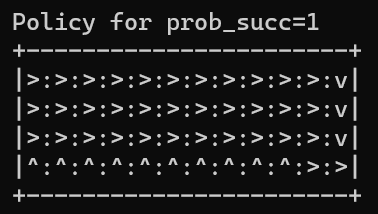
\includegraphics[width=\textwidth]{plots/proba10.png}
		\caption{Deterministic environment, $proba\_succ = 1$}
	\end{subfigure}
	\hfill
	\begin{subfigure}[b]{0.3\textwidth}
		\centering
		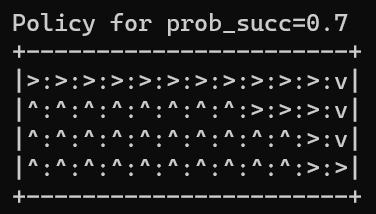
\includegraphics[width=\textwidth]{plots/proba07.png}
		\caption{Stochastic environment, $proba\_succ = 0.7$}
	\end{subfigure}
	\hfill
	\begin{subfigure}[b]{0.3\textwidth}
		\centering
		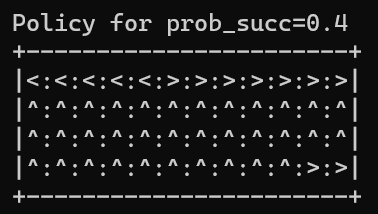
\includegraphics[width=\textwidth]{plots/proba04.png}
		\caption{Stochastic environment, $proba\_succ = 0.4$}
	\end{subfigure}
	\caption{Comparison of policies for the deterministic and the stochastic version of the environment.}
	\label{fig:policies}
\end{figure}


\subsection{}

Policy iteration has nested loops where it runs an inner loop of policy evaluation until convergence. It requires few iterations of the outer loop until convergence, although each of these policy evaluations is time-consuming.

Value iteration has only a single loop where it constantly updates the current V-function by acting greedily without evaluating a while policy. It does not wait for the whole policy evaluation. Therefore it requires many more iterations of this single outer loop but each of them is much quicker than for policy evaluation.

Moreover, let us analyze their complexity with respect to the size of the action set. Policy iteration preforms a maximization over the action set at each iteration of the outer loop, after a policy evaluation. Thus, it computes this maximization only a few times. Whereas value iteration performs the maximization over the action set at every iteration of the single loop is has. Since it requires many more iterations to converge, maximization over the action set can become a bottleneck for value iteration when the size of the action set is big.

In our case, the action set (size 4) is much smaller than the state space (size 48). As a result, value iteration appears to be much quicker to converge. Running time of both algorithms is compared in figure \ref{fig:running_time} and table \ref{table:running_time}, where value iteration is about thirty times as fast as policy iteration after being optimized using vectorization. It must be noted that policy iteration could not take fully advantage of vectorization. Yet, even without vectorization, value iteration remains about twice as quick as policy iteration.

In conclusion, policy iteration can be faster for very large action spaces, whereas value iteration is quicker for smaller action spaces. Also, the latter generally converges faster.

\begin{figure}[h!]
	\centering
	\begin{subfigure}[b]{0.45\textwidth}
		\centering
		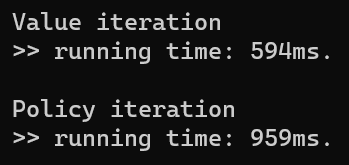
\includegraphics[width=0.7\textwidth]{plots/running_time.png}
		\caption{Using Python ``for'' loops}
	\end{subfigure}
	\hfill
	\begin{subfigure}[b]{0.45\textwidth}
		\centering
		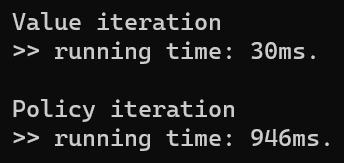
\includegraphics[width=0.7\textwidth]{plots/running_time_vect.png}
		\caption{Using vectorization for value iteration}
	\end{subfigure}
	\caption{Running time of value iteration and policy iteration in the deterministic version of the environment with the same tolerance toward convergence, best value over 20 runs.}
	\label{fig:running_time}
\end{figure}

\begin{table}[h!]
	\centering
	\begin{tabular}{||c c c||} 
		\hline
		Algorithm & Non vectorized & Vectorized \\ [0.5ex] 
		\hline\hline
		Policy iteration & 959 ms & 946 ms \\ 
		\hline
		Value iteration & 594 ms & 30 ms \\
		\hline
	\end{tabular}
	\caption{Running times of policy iteration and value iteration, best value over 20 runs.}
	\label{table:running_time}
\end{table}


\end{document}